% ============================================================
% GROUP TALK — 15 slides, ~12:30 content + 2:30 buffer = 15:00
% ============================================================

% ----------------------------------------------------------
% SLIDE 1: Title
% SAY: "I will show you a new framework for computing absorbed
%       power density on human bodies in wireless environments."
% ----------------------------------------------------------
\begin{frame}[plain]
  \vfill
  \begin{center}
    {\Large\color{navyblue}\bfseries Geometric dosimetry}\\[8pt]
    {\normalsize Closed-form absorption laws\\
     from \SI{100}{\mega\hertz} to \SI{100}{\giga\hertz}}\\[16pt]
    {\small Robin Wydaeghe}\\[2pt]
    {\footnotesize Ghent University \& imec}
  \end{center}
  \vfill
\end{frame}

% ----------------------------------------------------------
% SLIDE 2: The problem
% SAY: "At 28 GHz the skin depth is 0.3 mm but the body spans
%       a metre. To resolve absorption, FDTD needs 10^12 cells.
%       A single simulation takes weeks. A parametric study: months."
% ----------------------------------------------------------
\begin{frame}{The problem: FDTD at mmWave is intractable}

  \begin{columns}[T]
    \begin{column}{0.58\textwidth}
      The scale mismatch:
      \begin{itemize}
        \item Body span: ${\sim}\SI{1}{\metre}$
        \item Skin depth at \SI{28}{\giga\hertz}: $\delta \approx \SI{0.3}{\milli\metre}$
        \item Five orders of magnitude
      \end{itemize}

      \vspace{8pt}
      FDTD consequence:
      \begin{itemize}
        \item Mesh: ${\sim}10^{12}$ cells per simulation
        \item One plane wave, one phantom, one frequency: weeks
        \item Parametric campaign (550 runs): months of GPU
      \end{itemize}
    \end{column}

    \begin{column}{0.38\textwidth}
      \begin{center}
        \begin{tikzpicture}[scale=0.8]
          \draw[thick, navyblue] (0,0) -- (0,4);
          \draw[<->] (0.3,0) -- (0.3,4)
            node[midway,right] {\footnotesize $\SI{1}{\metre}$};
          \draw[thick, alertred, fill=alertred!20]
            (-0.04,3.94) rectangle (0.12,4);
          \draw[<->] (0.5,3.94) -- (0.5,4)
            node[midway,right] {\footnotesize $\delta \approx \SI{0.3}{\milli\metre}$};
          \node at (0,-0.5) {\footnotesize body};
          \node[alertred] at (0.8,4.3) {\footnotesize skin depth};
          \node[gray,rotate=90] at (-0.5,2) {\tiny not to scale ($3300{\times}$)};
        \end{tikzpicture}
      \end{center}
    \end{column}
  \end{columns}

  \vspace{6pt}
  \begin{resultbox}
    \centering
    We replace the volumetric simulation with surface-level geometric operations.
  \end{resultbox}
\end{frame}

% ----------------------------------------------------------
% SLIDE 3: Exact absorption law
% SAY: "Three factors. Illumination times material times geometry.
%       The equation is exact under a locally flat surface assumption.
%       The ReLU gate is exact: back-facing points absorb nothing.
%       Now, the interesting question: what happens to the red term?"
% ----------------------------------------------------------
\begin{frame}{Exact absorption law}

  Three factors determine local absorption:

  \vspace{8pt}
  \begin{center}
    {\large $\displaystyle
      \Sab(\rr) \;=\;
      \underbrace{{\color{colsinc}\Sinc}}_{\text{\scriptsize environment}}
      \;\cdot\;
      \underbrace{{\color{coltransmission}\Teff(\rr)}}_{\text{\scriptsize material}}
      \;\cdot\;
      \underbrace{{\color{colgeometry}\ReLU\!\bigl[\nhat(\rr)\cdot(-\khat)\bigr]}}_{\text{\scriptsize geometry}}
    $}
  \end{center}

  \vspace{10pt}
  \begin{columns}[T]
    \begin{column}{0.55\textwidth}
      \begin{itemize}
        \item {\color{colsinc}$\Sinc$}: incident power density
        \item {\color{coltransmission}$\Teff$}: Fresnel transmission, depends on\\
              angle, polarisation, tissue, frequency
        \item {\color{colgeometry}$\ReLU$}: visibility gate (exact).
              Back-facing points absorb nothing.
      \end{itemize}
    \end{column}

    \begin{column}{0.4\textwidth}
      \begin{center}
        
\includegraphics[width=0.9\textwidth]{incidence_plane_fig.pdf}
      \end{center}
    \end{column}
  \end{columns}

  \vspace{6pt}
  \hfill{\color{coltransmission}\small\bfseries What happens to the material factor?\hspace{12pt}}
\end{frame}

% ----------------------------------------------------------
% SLIDE 4: Pseudo-Brewster animation
% SAY: nothing (the animation narrates itself visually)
% ----------------------------------------------------------
\begin{frame}[plain]
  \centering
  \movie[width=\textwidth, height=0.5625\textwidth, autostart, once]{%
    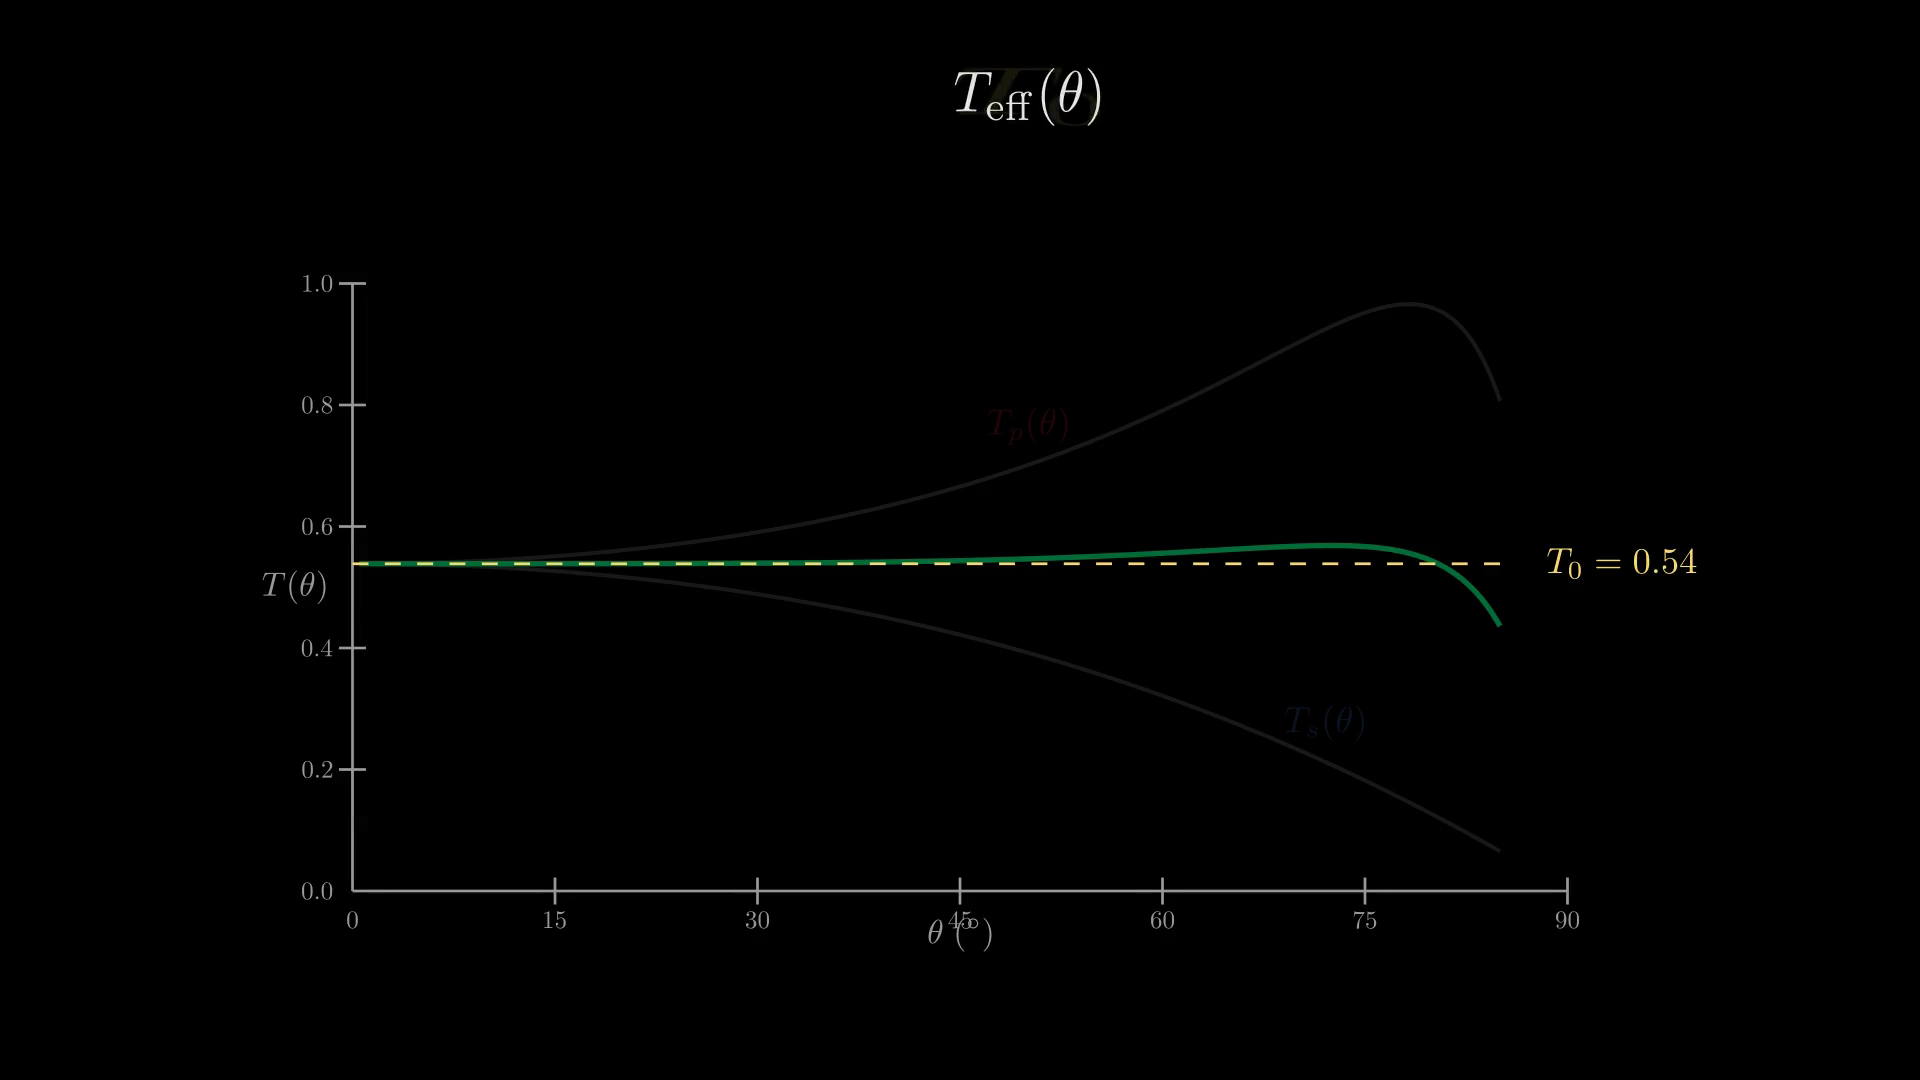
\includegraphics[width=\textwidth]{animations/poster_pseudo_brewster.png}%
  }{animations/PseudoBrewster.mp4}
\end{frame}

% ----------------------------------------------------------
% SLIDE 5: The geometric absorption law
% SAY: "The material factor collapses to a single number T_0.
%       All spatial variation is body geometry. That is the
%       geometric absorption law."
% ----------------------------------------------------------
\begin{frame}{The geometric absorption law}

  \begin{center}
    \vspace{6pt}
    Before: ${\color{coltransmission}\Teff(\theta, \mathrm{pol}, \mathrm{tissue}, f)}$
    \hspace{24pt}$\longrightarrow$\hspace{24pt}
    After: ${\color{coltransmission}T_0}$ (one number)

    \vspace{16pt}
    \begin{resultbox}[Geometric absorption law]
      \vspace{-4pt}
      {\large\[
        \Sab(\rr) \;\approx\;
        {\color{colsinc}\Sinc}
        \;\cdot\;
        {\color{coltransmission}T_0}
        \;\cdot\;
        {\color{colgeometry}\ReLU\!\bigl[\nhat(\rr)\cdot(-\khat)\bigr]}
      \]}
      \vspace{-6pt}
    \end{resultbox}
  \end{center}

  \vspace{12pt}
  \begin{columns}[T]
    \begin{column}{0.48\textwidth}
      {\small
      \begin{tabular}{lccr}
        \toprule
        Tissue & $|\ntilde|$ & $T_0$ & $\Tavg/T_0$ range \\
        \midrule
        Skin   & 4.84 & 0.54 & $\le 5.6\,\%$ \\
        Muscle & 5.62 & 0.48 & $\le 4.8\,\%$ \\
        Fat    & 2.05 & 0.77 & $\le 8.2\,\%$ \\
        \bottomrule
      \end{tabular}
      }
    \end{column}

    \begin{column}{0.48\textwidth}
      \begin{itemize}
        \item All spatial variation from body shape
        \item Holds for $|\ntilde| > 2.5$ (Azzam, 2015)
        \item Biological tissue: $|\ntilde| \approx 3$--6 \checkmark
      \end{itemize}
    \end{column}
  \end{columns}
\end{frame}

% ----------------------------------------------------------
% SLIDE 6: Geometry animation
% SAY: nothing (the animation narrates itself visually)
% ----------------------------------------------------------
\begin{frame}[plain]
  \centering
  \movie[width=\textwidth, height=0.5625\textwidth, autostart, once]{%
    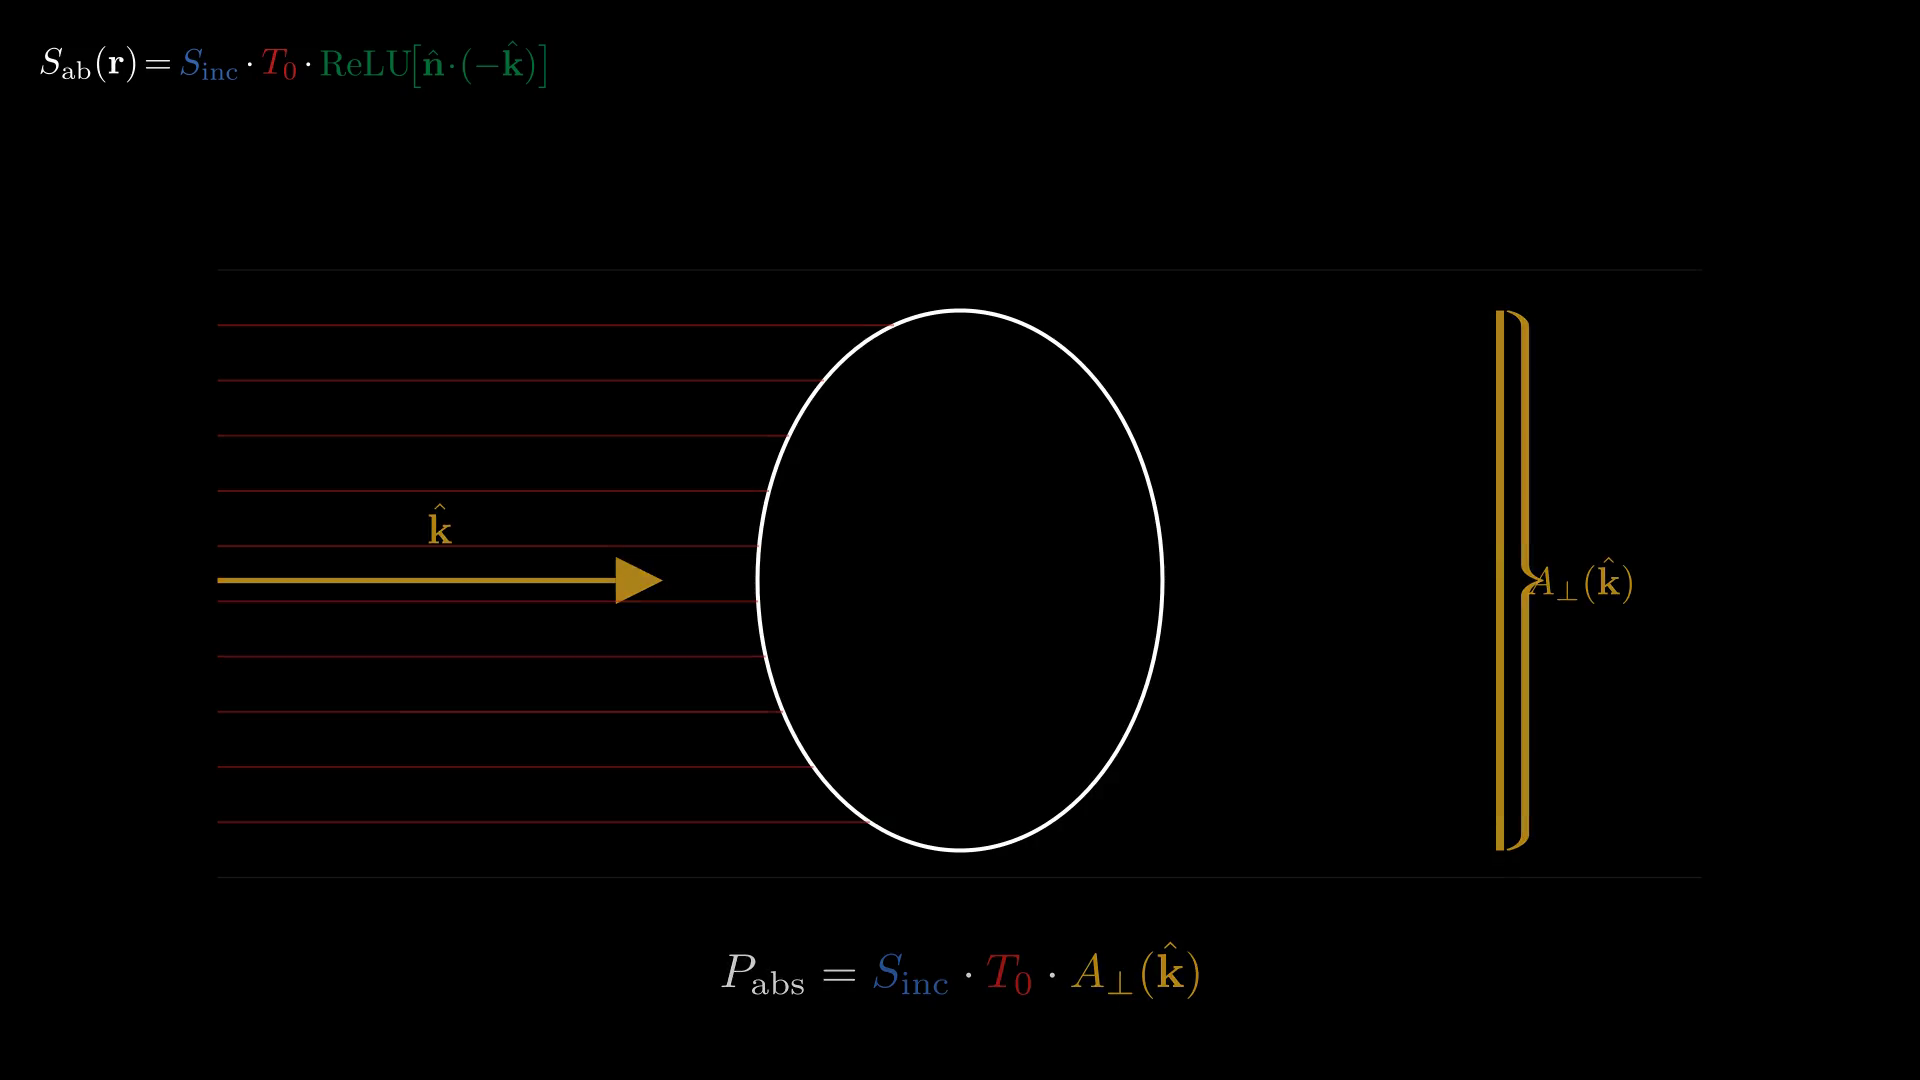
\includegraphics[width=\textwidth]{animations/poster_geometry.png}%
  }{animations/GeometryOfAbsorption.mp4}
\end{frame}

% ----------------------------------------------------------
% SLIDE 7: Validation
% SAY: "Mie theory tests both Fresnel and geometric optics.
%       Error is 5-10%, dominated by diffraction. The phantom
%       test isolates the Fresnel approximation: 0.35% error.
%       The framework error is smaller than tissue data uncertainty."
% ----------------------------------------------------------
\begin{frame}{Validation}

  \begin{columns}[T]
    \begin{column}{0.48\textwidth}
      \textbf{Mie theory} (exact for lossy spheres):
      \begin{itemize}
        \item Tests Fresnel + geometric optics jointly
        \item Body-scale at \SI{28}{\giga\hertz}: ${\sim}5$--$10\,\%$ error
        \item Dominated by diffraction into shadow
        \item Conservative (underestimates absorption)
      \end{itemize}

      \vspace{6pt}
      \textbf{Thelonious phantom}:
      \begin{itemize}
        \item Total absorbed power error: $0.35\,\%$
        \item Local RMS: $3.2\,\%$
      \end{itemize}
    \end{column}

    \begin{column}{0.48\textwidth}
      \begin{center}
        
\includegraphics[width=\textwidth]{mie_panel_a.png}\\[2pt]
        {\footnotesize Error vs size parameter at \SI{28}{\giga\hertz}.\\
         Body parts annotated by diameter.}
      \end{center}
    \end{column}
  \end{columns}

  \vspace{4pt}
  \begin{resultbox}
    \centering
    Framework error (5--15\,\%) $<$ tissue dielectric uncertainty (${\sim}20\,\%$).\\
    The data is less accurate than the model.
  \end{resultbox}
\end{frame}

% ----------------------------------------------------------
% SLIDE 8: Speed and computation
% SAY: "Six orders of magnitude. 550 parametric runs take
%       milliseconds on a laptop. The dosimetry chain is a
%       single-hidden-layer ReLU network, differentiable end to end."
% ----------------------------------------------------------
\begin{frame}{Speed}

  \begin{center}
    \vspace{12pt}
    {\Huge\color{resultgreen}\bfseries $10^6\times$}\\[6pt]
    {\large speedup over full-wave FDTD}

    \vspace{16pt}
    {\normalsize
      550 parametric runs: milliseconds on a laptop.\\
      Previously: months of GPU time.
    }

    \vspace{16pt}
    \begin{resultbox}[Dosimetry as a ReLU network]
      \vspace{-6pt}
      \[
        \mathbf{S}_{\mathrm{ab}} = {\color{coltransmission}T_0}
        \;{\color{colgeometry}\ReLU(\NN\KK^\top)}\;
        {\color{colsinc}\ssv}
      \]
      \vspace{-8pt}
    \end{resultbox}
    {\small Single hidden layer. Differentiable end to end.\\
     Gradients of SAR w.r.t.\ antenna positions by backpropagation.}
  \end{center}
\end{frame}

% ----------------------------------------------------------
% SLIDE 9: Demo intro
% SAY: "Let me show you."
% ----------------------------------------------------------
\begin{frame}[plain]
  \vfill
  \begin{center}
    {\Huge\color{navyblue}\bfseries AEGIS}\\[8pt]
    {\large Real-time geometric dosimetry}\\[16pt]
    {\normalsize
      3D viewer\quad$\mid$\quad
      9 fidelity levels\quad$\mid$\quad
      ray tracing\quad$\mid$\quad
      ICNIRP compliance
    }
  \end{center}
  \vfill
\end{frame}

% ----------------------------------------------------------
% SLIDE 10: Live demo
% SAY: (live demo of AEGIS viewer, ~2 minutes)
% ----------------------------------------------------------
\begin{frame}[plain]
  \vfill
  \begin{center}
    {\color{darkgray}\Large Live demo}
  \end{center}
  \vfill
\end{frame}

% ----------------------------------------------------------
% SLIDE 11: Bridge to coherent MIMO
% SAY: "Everything so far assumed incoherent illumination.
%       Powers add. In MIMO, fields add. The coherent peak
%       can exceed the incoherent sum by a factor N."
% ----------------------------------------------------------
\begin{frame}{From incoherent to coherent}

  \begin{columns}[c]
    \begin{column}{0.45\textwidth}
      \begin{center}
        {\bfseries\color{navyblue} Parts I--II: incoherent}\\[6pt]
        Powers add.\\[4pt]
        $P_{\mathrm{abs}} = \sum_n P_n$\\[6pt]
        Cross-terms average to zero.
      \end{center}
    \end{column}

    \begin{column}{0.08\textwidth}
      \begin{center}
        {\Large$\longrightarrow$}
      \end{center}
    \end{column}

    \begin{column}{0.45\textwidth}
      \begin{center}
        {\bfseries\color{alertred} Part III: coherent MIMO}\\[6pt]
        Fields add.\\[4pt]
        $\EE_{\mathrm{tot}} = \sum_m x_m \EE_m$\\[6pt]
        Peak absorption: ${\color{alertred}N^2}$ vs $N$.
      \end{center}
    \end{column}
  \end{columns}

  \vspace{16pt}
  \begin{center}
    {\small $M$ antenna elements, precoding vector $\xx \in \Complex^M$.\\
     The signal branch collapses each path to a scalar at the UE.\\
     The exposure branch retains the full vector structure over the body surface.}
  \end{center}
\end{frame}

% ----------------------------------------------------------
% SLIDE 12: Coherent phasor animation
% SAY: nothing (the animation narrates itself visually)
% ----------------------------------------------------------
\begin{frame}[plain]
  \centering
  \movie[width=\textwidth, height=0.5625\textwidth, autostart, once]{%
    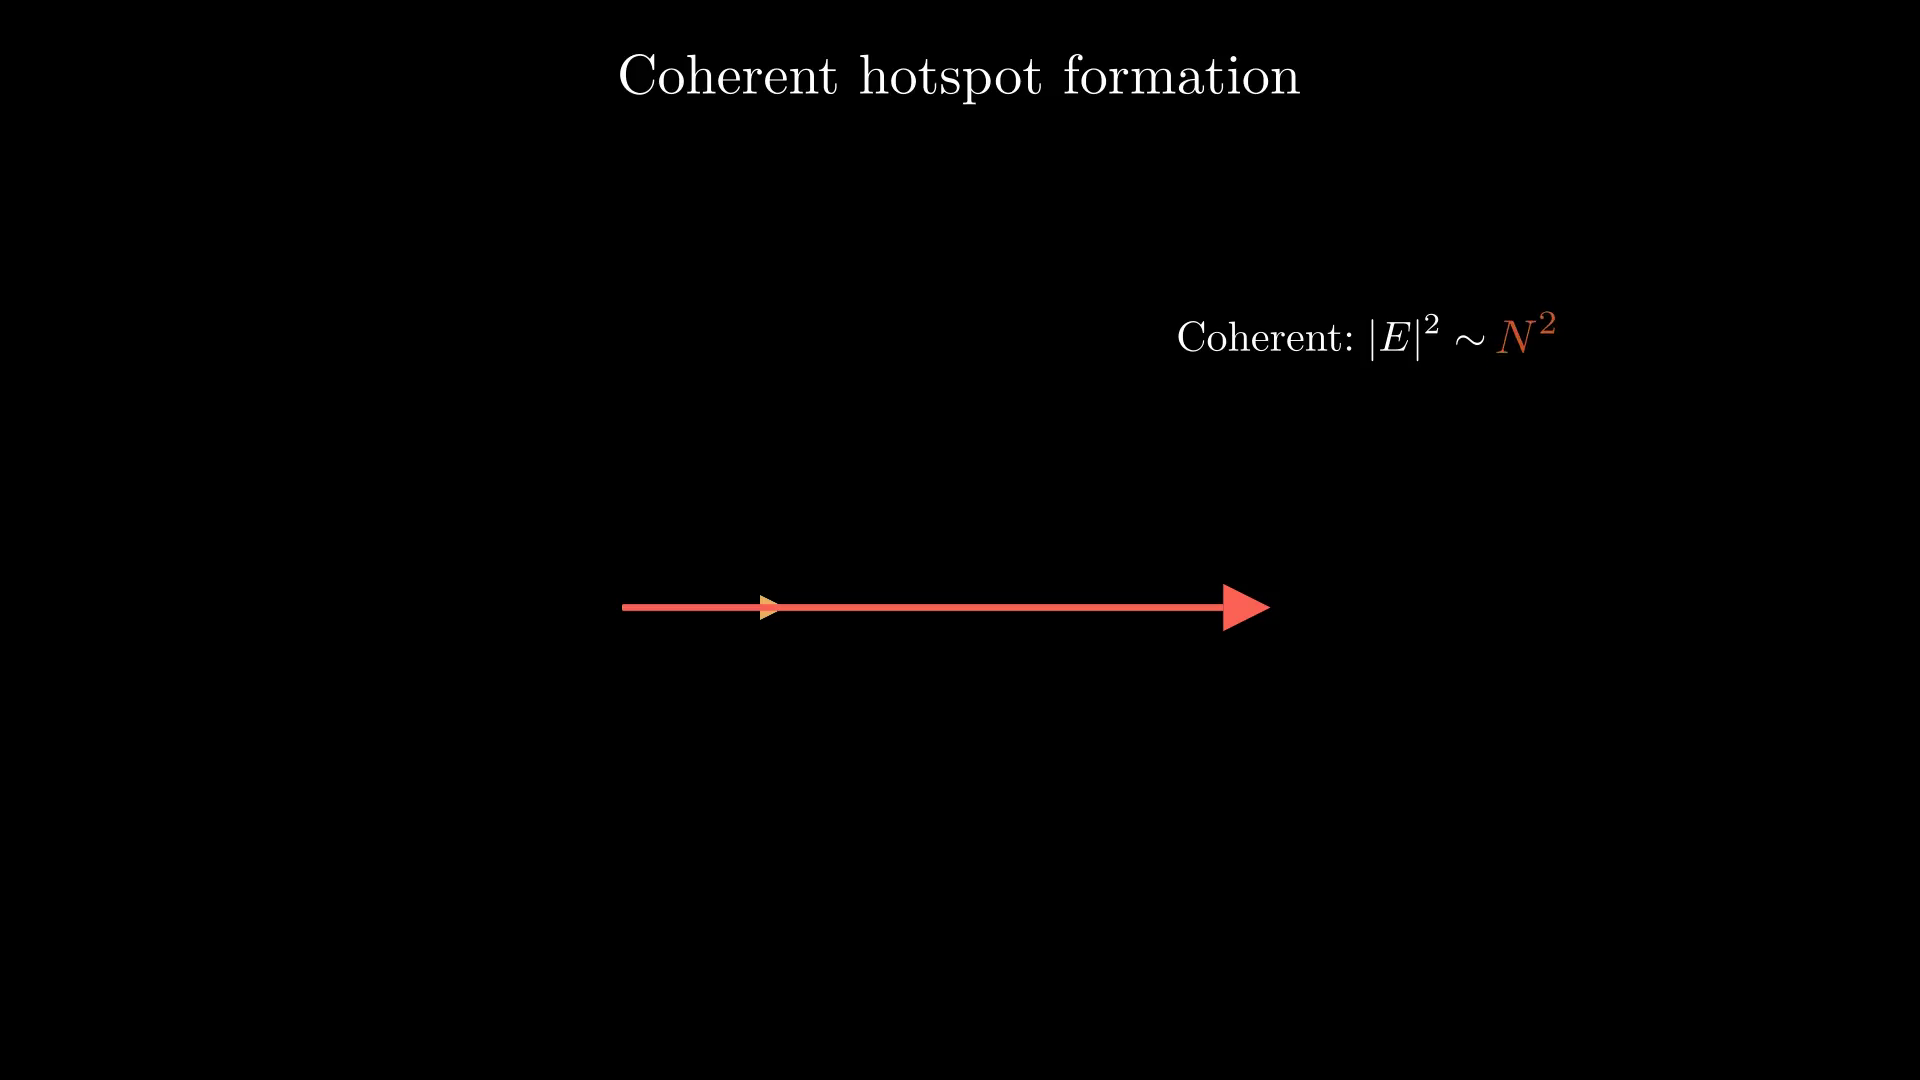
\includegraphics[width=\textwidth]{animations/poster_coherent.png}%
  }{animations/CoherentPhasors.mp4}
\end{frame}

% ----------------------------------------------------------
% SLIDE 13: Exposure operator and ECBF
% SAY: "Integrate the squared norm over the body surface and
%       you get a quadratic form. Q is Hermitian PSD, M by M.
%       The optimization is a QCQP with a closed-form solution.
%       The inverse suppresses high-absorption modes."
% ----------------------------------------------------------
\begin{frame}{Exposure-constrained beamforming}

  Coherent absorption law and exposure operator:

  \vspace{4pt}
  \begin{columns}[T]
    \begin{column}{0.48\textwidth}
      \begin{resultbox}[Coherent absorption law]
        \vspace{-6pt}
        \[
          \Sab(\rr) = \bigl\|\Gtilde(\rr)\,\xx\bigr\|^2
        \]
        \vspace{-8pt}
      \end{resultbox}

      \vspace{4pt}
      \begin{resultbox}[Exposure operator]
        \vspace{-6pt}
        \[
          P_{\mathrm{abs}} = \xx^H \QQ\, \xx
        \]
        \vspace{-10pt}
        \[
          \QQ = \int_\Sigma \Gtilde^H \Gtilde\,\diff A
          \;\in\; \Complex^{M \times M}
        \]
        \vspace{-8pt}
      \end{resultbox}
    \end{column}

    \begin{column}{0.48\textwidth}
      Maximise signal subject to absorption limit:
      \[
        \max_{\xx} \;|\hh^\top \xx|^2
        \;\;\text{s.t.}\;\;
        \xx^H \QQ\, \xx \le P_{\mathrm{abs}}^{\max}
      \]

      \vspace{2pt}
      Closed-form solution (S-procedure):
      \[
        \xx^\star = \sqrt{P}\;
        \frac{(\lambda\QQ + \nu\II)^{-1}\hh^*}
             {\|(\lambda\QQ + \nu\II)^{-1}\hh^*\|}
      \]

      \vspace{6pt}
      {\footnotesize
        $\lambda = 0$: MRT (unconstrained).\\
        $\lambda \gg \nu$: body-avoiding precoder.\\
        $\rho \ll 1$: natural geometric protection.
      }
    \end{column}
  \end{columns}
\end{frame}

% ----------------------------------------------------------
% SLIDE 14: Summary
% SAY: "Three results. Material physics makes dosimetry geometric.
%       The geometry is fast. The fast computation enables
%       exposure-aware network design."
% ----------------------------------------------------------
\begin{frame}{Summary}

  \vspace{4pt}
  The equation chain:
  \begin{align*}
    \text{Exact:}\quad & \Sab = {\color{colsinc}\Sinc} \cdot {\color{coltransmission}\Teff(\theta)} \cdot {\color{colgeometry}\ReLU[\nhat\!\cdot\!(-\khat)]} \\[4pt]
    \xrightarrow{\text{pseudo-Brewster}}\quad & \Sab \approx {\color{colsinc}\Sinc} \cdot {\color{coltransmission}T_0} \cdot {\color{colgeometry}\ReLU[\nhat\!\cdot\!(-\khat)]} \\[4pt]
    \xrightarrow{\text{coherent}}\quad & \Sab = \|\Gtilde\,\xx\|^2, \qquad P_{\mathrm{abs}} = \xx^H\QQ\,\xx
  \end{align*}

  \vspace{4pt}
  \begin{columns}[T]
    \begin{column}{0.3\textwidth}
      \begin{center}
        {\small\bfseries\color{coltransmission} Material}\\[4pt]
        {\footnotesize
          Pseudo-Brewster:\\
          $\Teff \to T_0$\\
          One number per tissue.
        }
      \end{center}
    \end{column}

    \begin{column}{0.3\textwidth}
      \begin{center}
        {\small\bfseries\color{colgeometry} Geometry}\\[4pt]
        {\footnotesize
          $\Sab \propto \ReLU(\cos\theta)$\\
          Shadow area, Cauchy formula.\\
          $10^6\times$ speedup.
        }
      \end{center}
    \end{column}

    \begin{column}{0.3\textwidth}
      \begin{center}
        {\small\bfseries\color{navyblue} Coherent MIMO}\\[4pt]
        {\footnotesize
          $\QQ = \int \Gtilde^H\Gtilde\,\diff A$\\
          Closed-form ECBF.\\
          Exposure-aware design.
        }
      \end{center}
    \end{column}
  \end{columns}

  \vspace{10pt}
  \begin{center}
    {\small Tissue physics makes dosimetry geometric.
     The geometry is fast.\\
     The fast computation enables exposure-aware network design.}
  \end{center}
\end{frame}

% ----------------------------------------------------------
% SLIDE 15: Thank you
% ----------------------------------------------------------
\begin{frame}[plain]
  \vfill
  \begin{center}
    {\Large\color{navyblue}\bfseries Thank you}\\[12pt]
    {\normalsize Questions and discussion}\\[16pt]
    {\footnotesize Robin Wydaeghe \quad$\mid$\quad robin.wydaeghe@ugent.be}
  \end{center}
  \vfill
\end{frame}
